\documentclass[10pt,final,a4paper,oneside,onecolumn]{article}

%%==========================================================================
%% Packages
%%==========================================================================
\usepackage[a4paper,left=3.5cm,right=3.5cm,top=3cm,bottom=3cm]{geometry} %% change page layout; remove for IEEE paper format
\usepackage[T1]{fontenc}                        %% output font encoding for international characters (e.g., accented)
\usepackage[cmex10]{amsmath}                    %% math typesetting; consider using the [cmex10] option
\usepackage{amssymb}                            %% special (symbol) fonts for math typesetting
\usepackage{amsthm}                             %% theorem styles
\usepackage{dsfont}                             %% double stroke roman fonts: the real numbers R: $\mathds{R}$
\usepackage{mathrsfs}                           %% formal script fonts: the Laplace transform L: $\mathscr{L}$
\usepackage[pdftex]{graphicx}                   %% graphics control; use dvips for TeXify; use pdftex for PDFTeXify
\usepackage{array}                              %% array functionality (array, tabular)
\usepackage{upgreek}                            %% upright Greek letters; add the prefix 'up', e.g. \upphi
\usepackage{stfloats}                           %% improved handling of floats
\usepackage{multirow}                           %% cells spanning multiple rows in tables
%\usepackage{subfigure}                         %% subfigures and corresponding captions (for use with IEEEconf.cls)
\usepackage{subfig}                             %% subfigures (IEEEtran.cls: set caption=false)
\usepackage{fancyhdr}                           %% page headers and footers
\usepackage[official,left]{eurosym}             %% the euro symbol; command: \euro
\usepackage{appendix}                           %% appendix layout
\usepackage{xspace}                             %% add space after macro depending on context
\usepackage{verbatim}                           %% provides the comment environment
\usepackage[dutch,USenglish]{babel}             %% language support
\usepackage{wrapfig}                            %% wrapping text around figures
\usepackage{longtable}                          %% tables spanning multiple pages
\usepackage{pgfplots}                           %% support for TikZ figures (Matlab/Python)
\pgfplotsset{compat=1.14}						%% Run in backwards compatibility mode
\usepackage[breaklinks=true,hidelinks,          %% implement hyperlinks (dvips yields minor problems with breaklinks;
bookmarksnumbered=true]{hyperref}   %% IEEEtran: set bookmarks=false)
%\usepackage[hyphenbreaks]{breakurl}            %% allow line breaks in URLs (don't use with PDFTeX)
\usepackage[final]{pdfpages}                    %% Include other pdfs
\usepackage[capitalize]{cleveref}				%% Referensing to figures, equations, etc.
\usepackage{units}								%% Appropriate behavior of units
\usepackage[utf8]{inputenc}   				 	%% utf8 support (required for biblatex)
\usepackage{csquotes}							%% Quoted texts are typeset according to rules of main language
\usepackage[style=ieee,doi=false,isbn=false,url=false,date=year,minbibnames=15,maxbibnames=15,backend=biber]{biblatex}
%\renewcommand*{\bibfont}{\footnotesize}		%% Use this for papers
\setlength{\biblabelsep}{\labelsep}
\bibliography{../../bib}

%%==========================================================================
%% Define reference stuff
%%==========================================================================
\crefname{figure}{Figure}{Figures}
\crefname{equation}{}{}

%%==========================================================================
%% Define header/title stuff
%%==========================================================================
\newcommand{\progressreportnumber}{21}
\renewcommand{\author}{Erwin de Gelder}
\renewcommand{\date}{August 1, 2019}
\renewcommand{\title}{Performance assessment of automated vehicles using real-world driving scenarios}

%%==========================================================================
%% Fancy headers and footers
%%==========================================================================
\pagestyle{fancy}                                       %% set page style
\fancyhf{}                                              %% clear all header & footer fields
\fancyhead[L]{Progress report \progressreportnumber}    %% define headers (LE: left field/even pages, etc.)
\fancyhead[R]{\author, \date}                           %% similar
\fancyfoot[C]{\thepage}                                 %% define footer

\begin{document}
	
\begin{center}
	\begin{tabular}{c}
		\title \\ \\
		\textbf{\huge Progress report \progressreportnumber} \\ \\
		\author \\ 
		\date
	\end{tabular}
\end{center}

\section{Previous meeting minutes}

\begin{itemize}
	\item We discussed the graduate school credits. I still need a few credits for the transferable skills. See ``Future plans'', \cref{sec:future}.
	\item We discussed some preliminary work on risk quantification. More on this in ``Summary of work''.
\end{itemize}

\section{Summary of work}

\begin{itemize}
	\item I got feedback on the ontology paper from Hala Elrofai, Jan-Pieter Paardekooper, Olaf Op den Camp, and Jeroen Ploeg. Most feedback is processed. Most important thing to do is to improve the introduction and conclusion, such that it is more convincing that the ontology is really helpful regarding the assessment of automated vehicles.
	%\begin{itemize}
	%	\item I want to make a connection to the work we do in an ISO working group where the goal is to define the different attributes of a scenario and different ``scenario categories'' (a scenario category is similar to a ``scenario class'' in the ontology paper).
	%	\item I want to improve the conclusion, such that it is more convincing that the ontology is really helpful regarding the assessment of automated vehicles.
	%	\item 
	%\end{itemize}
	\item I worked out some more details of the risk quantification of a scenario class. I attached a small report.
\end{itemize}

\section{Future plans}
\label{sec:future}

\begin{itemize}
	\item In the previous meeting, I mentioned that I already have the required 15 graduate school credits for the discipline-related skills. I will obtain the 15 credits for the research-related skills using the learning-on-the-job activities. I also mentioned that I have 7.5 credits for the transferable skills. This means that I need 7.5 more credits for the transferable skills.
	
	I actually have now 11 credits for the transferable skills. The 0.5+1+2 credits for the courses \emph{PhD startup A}, \emph{How to become effective in a network conversation}, and \emph{Communication, Coping-strategies \& Awareness}.
	
	For the remaining 4 credits, I have the following plan:
	\begin{itemize}
		\item 1 credit for the \emph{PhD Career development} (required course near the end of the PhD).
		\item 3 credits for \emph{Writing a Dissertation}. I heard good review about this course. Furthermore, during this course, the introduction of the PhD dissertation will be written, so the time will be well spent.
	\end{itemize}
	\item During the Go/No Go meeting, I prepared a planning regarding my publications, see \cref{fig:old planning}. This planning is outdated. I propose a new planning, see \cref{fig:new planning}. Some remarks concerning the proposed planning:
	\begin{itemize}
		\item It seemed that I am rather inactive in Q3 and Q4 of year 2, as I am only working on the papers about the ontology and the scenario risk quantification. This can be explained by the fact that I spent quite significant time to non-PhD related matters.
		\item Q1 and Q2 of year 3 seem rather ambitious, as there are four topics to work on. In case the ontology paper is not finished yet, there are five topics to work on. Therefore, it is questionable whether this is realistic. Perhaps I have to drop or postpone one topic. 
	\end{itemize}

	\begin{figure}
		\centering
		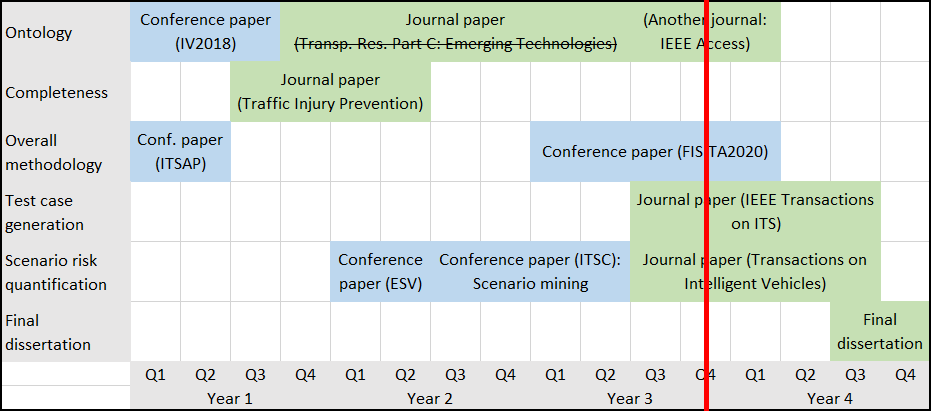
\includegraphics[width=\linewidth]{../../"20180917 GoNoGo"/figures/planning}
		\caption{Planning at the time of the Go/No Go meeting. The red line indicates the time at that moment.}
		\label{fig:old planning}
	\end{figure}
	
	\begin{figure}
		\centering
		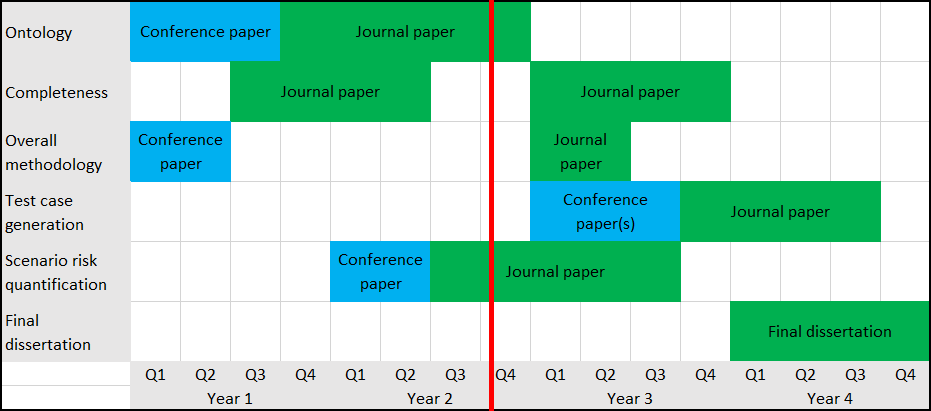
\includegraphics[width=\linewidth]{figures/planning}
		\caption{Proposed planning of my publications. The red line indicates the time of writing this report (i.e., almost at the start of year 3).}
		\label{fig:new planning}
	\end{figure}

	Some comments for each of the topics I want to write a paper for:
	\begin{itemize}
		\item \emph{Ontology for scenarios for the assessment of AVs.} This paper is almost ready to be submitted.
		\item \emph{Quantifying completeness of scenarios.} According to the original planning, I wanted to write a conference paper first. However, it ended up being a special issue of a journal \cite{degelder2019completeness}. Still, I consider it unfinished work, so I want to continue the work on this topic. 
		\item {Overal methodology: Framework for the safety assessment of AVs}. I have been busy with this within CETRAN, the project in Singapore. The project will be extended by half a year, so I can still work on it during Q1 and Q2 of year 3. I think this work could be a nice way to give all other work good context. However, I have my doubts if we can make this into a journal publication:
		\begin{itemize}
			\item First, in Singapore, they are very reluctant with publishing any information about the overall methodology.
			\item Secondly, the quality of the current work is probably not enough ``science based''.
		\end{itemize}
		\item \emph{Test case generation for the assessment of AVs.} This work includes the parametrization of the scenarios and the estimation of the probability density functions. Additionally, this work should describe how critical test cases (i.e., test cases for which the performance of the AV might be critical) can be generated.
		\item \emph{Risk quantification for scenario classes for automated driving systems.} This should extend the work done in the conference paper about this topic \cite{degelder2019risk}.
		\item \emph{Final dissertation.} I aim for a ``paper-based'' dissertation. I have no idea how much time it takes to write the actual dissertation, so I estimated it to take a year.
	\end{itemize}
\end{itemize}

%\section{Questions}
%
%\begin{itemize}
%	\item 
%\end{itemize}


\printbibliography

\clearpage
\includepdf[pages=-,pagecommand={},width=\paperwidth]{../../"20190725 Scenario Risk"/scenariorisk.pdf}

\end{document}